\chapter{PerfCake}\label{perfcake}
\setcounter{page}{1}
\pagenumbering{arabic}

Táto kapitola sa venuje nástroju na testovanie výkonu PerfCake, jeho použitiu a typu dát, ktorými sa budeme zaoberať. Celá kapitola je len povrchným zoznámením sa s nástrojom pre potreby tejto práce, čerpá hlavne z oficiálne stránky tohto nástroja, kde v prípade väčšieho záujmu je všetko o nástroji podrobne rozpísané.

\begin{figure}[ht]

\includegraphics[scale=1]{blog-logo.png}
\caption{PerfCake}
\end{figure} 

\section{O nástroji}

PerfCake je open-source framework vyvíjaný spoločnosťou Red Hat. Je to generátor zaťaženia s cieľom byť minimalistický a ľahko ovládateľný, poskytujúci stabilné výsledky, majúci minimálny vplyv na testovaný systém, byť nezávislý na platforme, umožňujúci vysokú priepustnosť a používajúci komponentový dizajn.

Nástroj PerfCake môže byť použitý na na všetky druhy testovania výkonu, včetne: 
\begin{itemize}  
\item \textit{záťažové testovanie (load testing)} - testuje sa správanie softvéru pri očakávanom zaťažení, pri tomto type testu sa prejavujú takzvané ``hrdlá fľaše''(\textit{bottlenecks}) v sytéme, miesta, ktoré v nejakom smere sytém limitujú,
\item \textit{testovanie hraničnej záťaže (stress testing)}- tento test hľadá hranice možného zaťaženia systému a zisťuje správanie sa systému za touto hranicou,
\item \textit{testovanie odolnosti (endurance testing, soak testing)} - zisťuje sa, či testovaný systém dokáže vydržať sústavnú záťaž po dlhšiu dobu a taktiež, či pri takejto sústavnej záťaži neklesá jeho výkon,
\item \textit{testovanie škálovateľnosti (scalability testing)} - testuje sa, či systém dobre škáluje a teda či je možné efektívne zvyšovať jeho kapacity bez zmien nečakaných správania,
\item \textit{benchmarking} - zaznamenávanie a porovnávanie výsledkov testov, za účelom získania rôznych metrík.
\end{itemize}

Pre účely spomínaných testov, podporuje PerfCake radu metrík na testovanie cieľového systému. Napríklad:
\begin{itemize}
\item monitorovanie vybraného atribútu správy, roztriedenie a spočítanie podľa konkrétnych hodnôt daného atribútu,
\item počítanie priemernej priepustnosti za sekundu,
\item sledovanie veľkosti spotrebovanej pamäte cieľovej JVM (Java virtual machine),
\item zaznamenávanie času odpovede (response time) v milisekundách, pomocou HDR (High Dynamic Range) histogramu, ktorý dokáže riešiť problém Koordinovaného vynechania (Coordinated ommission), viac o tomto probléme a riešení pomocou HRD histogramu sa môžme dočítať na oficiálnej stránke nástroja v sekcii 4.7. Reporting [],
\item počítanie štatistík, ako maximum, minimum, priemer z hodnôt priepustnosti alebo časov odpovedí, za čas od začiatku trvania testu, až po reportovanie výsledku alebo zo špecifikovaného časového okna,
\item detekovanie pripravenosti systému, ktorá sa určuje pomocou splnenia 3 podmienok, momentálna priepustnosť sa mení o menej ako nastaviteľná hranica, špecifikovaný čas bol dosiahnutý a špecifikovaný počet iterácií bol vykonaný,
\item  rozoznávanie geo-lokácie tretích strán.
\end{itemize}

Užívateľ má niekoľko možností reportovania výsledkov, ako napríklad výpis na konzolu, súbor logov, CSV formát, ktorý môže byť importovaný ako tabuľkový zošit (\textit{spreadsheet}) pomocou nástrojov ako Excel alebo LibreOffice Calc, alebo tiež dokáže generovať grafy výsledkov už v priebehu testovania. 
%Nástroj poskytuje viac možností výsledkov, vrátane priemernej priepustnosti alebo veľkosti spotrebovanej pamäte cieľovej JVM (Java virtual machine), s možnosťou regresnej analýzy za účelom odhalenia úniku pamäte.

Jeden z problémov podobných testovacích nástrojov je prípad, kedy testovaný softvér zlyhá a vzápätí odošle chybovú správu. Pre tento prípad sú v nástroji PerfCake zabudované validátory, ktoré dokážu takúto správu rozpoznať a nezaviesť tým chybové správy do výsledku výkonu softvéru. Podobné softvéry, ktoré takéto validácie neprevádzajú potom vytvárajú veľmi skreslený výsledok.

\section{Použitie}

Pre spustenie nástroja PerfCake je potrebné vytvoriť, takzvané scenáre (scenarios). V týchto súboroch sú definované testovacie bloky, ktoré hovoria PerfCaku čo a ako robiť. Scenáre sú rozdelené do niekoľko sekcií:
\begin{itemize}
\item \textit{vlastnosti (properties)} - táto sekcia slúži na pridanie akýchsi meta-dát o scenári, nie je to povinný parameter a slúži na komplexnejšie využitie testovacích scenárov,
\item \textit{beh (run)} - slúži na  definovanie dĺžky trvania testu,
\item \textit{generátor (generator)} - špecifikuje ako a koľko zaťaženia sa má vytvárať,
\begin{figure}[!ht]
\centering
\includegraphics[width=0.65\linewidth]{scenarioStructure.png} 
\caption{Štruktúa scenára}\label{scenarioStructure}
\end{figure}
\item \textit{odosielateľ (sender)} - táto sekcia je o spôsobe prenosu, o tom, kde zaťaženie posielať, poprípade o prijímaní odozvy z testovaného systému,
\item \textit{prijímateľ (receiver)} - ďalšia rozširujúca sekcia, ktorá sa používa v prípade, že odozva z testovaného systému prichádza iným kanálom (protokolom) ako bola poslaná správa,
\item \textit{reportovanie (reporting)} - definuje metriky, spôsob a výstup reportovania výsledkov testu,
\item \textit{správy (messages)} -  sekcia slúži na definovanie formátu a obsahu správ posielaných na testovaný systém,
\item \textit{sekvencie (sequencies)} - táto sekcia umožňuje používať sekvenciu hodnôt, ktoré sa menia pre každú správu (prípadne množinu správ, špecifikovaných v jednom scenári), čo dáva možnosť vytvárať unikátne správy,
\item \textit{validácia (validation)} - dovoľuje validovať odpoveď  testovaného systému.
\end{itemize}

Štruktúru testovacieho scenára vo formáte XML (eXtensible Markup Language) a povinnosť konkrétnych parametrov zobrazuje obrázok \ref{scenarioStructure}. Okrem tohto formátu podporuje PerfCake aj iné možnosti scenárov, napríklad DSL (Domain Specific Language) formát alebo použitie špeciálneho rozhrania pre programovanie aplikácií (API) v jazyku Java, kde si užívateľ môže nadefinovať celý scenár.
%Validátory sa konfigurujú spolu s podobou správ, ktoré má nástroj odosielať na cieľový softvér. Takáto validácia sa rovnako ako scenáre, píše vo formáte XML.


%\begin{wrapfigure}{l}{0.6\textwidth}
%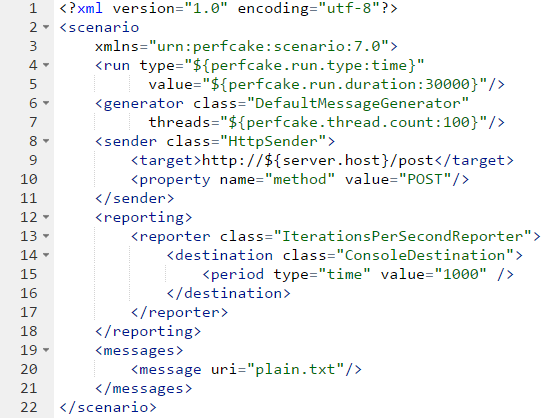
\includegraphics[width=0.9\linewidth]{scenario.png} 
%\caption{Príklad scenára}\label{scenario}
%\end{wrapfigure}

\begin{figure} [!htb]
\centering
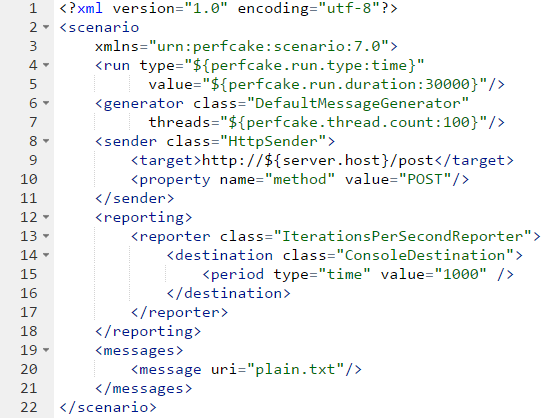
\includegraphics[width=0.9\linewidth]{scenario.png} 
\caption{Príklad scenára}\label{scenario}
\end{figure}
Pre jednoduchú ukážku si uvedieme príklad scenára XML. Máme vyvinutý softvér, ktorý asynchrónne spracováva správy prichádzajúce pomocou POST metódy a HTTP protokolu. Následne tieto správy spracúva (validuje, vytvára záznamy do databázy, generuje reporty, ...) a po úspešnom spracovaní pošle potvrdzujúcu správu späť.
Na obrázku \ref{scenario} sa nachádza scenár pre jednoduchý testovací blok, ktorý by sme mohli na takýto nami vytvorený softvér použiť. Zo scenára je možné vidieť, že tento test bude bežať 3000 ms = 3 sekundy, generuje správy použitím 100 vlákien, ktoré posiela pomocou HTTP protokolu a metódy POST. Text správy je špecifikovaný v súbore``plain.txt'' a výsledky sú zaznamenávané na konzolu, každú 1 sekundu. Ako reporter je použitý ``IterationsPerSecondReporter'' a teda sa každú sekundu zapíše, koľko správ bolo softvérom spracovaných. 

Veľmi podobným scenárom by sme mohli testovať, koľko softvér používa pamäte, stačilo by zmeniť atribút reporter na ``MemoryUsageReporter''. Týmto spôsobom sa veľmi ľahko odhaľujú úniky pamäte. Scenáre sa púšťajú pomocou nástroja Maven alebo pomocou shell skriptu.



\section{Výstup}

Ako bolo uvedené v prvej podkapitole, PerfCake má bohaté možnosti východzích súborov. Pri vytváraní optimalizačného algoritmu budeme ale pracovať iba s dvoma typmi. Dáta budeme spracovávať z CSV súboru a následne z nich budeme generovať grafy. 

\begin{table}[!htb]
\centering
\begin{tabular}{|l|l|l|l|l|l|}
\hline
\multicolumn{3}{|c|}{\textit{\textbf{Throughput}}}  & \multicolumn{3}{c|}{\textit{\textbf{Memory}}}  \\ \hline
\textbf{Time} & \textbf{Current} & \textbf{Average} & \textbf{Time} & \textbf{Used} & \textbf{Total} \\ \hline
00:01:00      & 1,67             & 1,67             & 00:01:00      & 777,30        & 2817,06        \\ \hline
00:02:00      & 1,67             & 1,67             & 00:02:00      & 528,81        & 2835,94        \\ \hline
00:03:00      & 2,22             & 2,22             & 00:03:00      & 450,90        & 2901,19        \\ \hline
00:04:00      & 2,08             & 2,08             & 00:04:00      & 585,94        & 2911,63        \\ \hline
00:05:00      & 2,33             & 2,33             & 00:05:00      & 979,96        & 2953,00        \\ \hline
00:06:00      & 2,22             & 2,22             & 00:06:00      & 855,63        & 2960,25        \\ \hline
00:07:00      & 2,38             & 2,38             & 00:07:00      & 1193,20       & 2992,13        \\ \hline
00:08:00      & 2,29             & 2,29             & 00:08:00      & 1175,80       & 3001,75        \\ \hline
00:09:00      & 2,22             & 2,22             & 00:09:00      & 1197,66       & 3009,88        \\ \hline
00:10:00      & 2,17             & 2,17             & 00:10:00      & 831,64        & 3013,38        \\ \hline
00:11:00      & 2,27             & 2,27             & 00:11:00      & 1380,88       & 3019,63        \\ \hline
00:12:00      & 2,22             & 2,22             & 00:12:00      & 815,44        & 3031,56        \\ \hline
00:13:00      & 2,18             & 2,18             & 00:13:00      & 950,54        & 3035,38        \\ \hline
00:14:00      & 2,26             & 2,26             & 00:14:00      & 726,44        & 3036,44        \\ \hline
00:15:00      & 2,44             & 2,33             & 00:15:00      & 659,87        & 3042,88        \\ \hline
00:16:00      & 2,18             & 2,19             & 00:16:00      & 715,86        & 3042,88        \\ \hline
00:17:00      & 2,18             & 2,16             & 00:17:00      & 909,47        & 3042,44        \\ \hline
00:18:00      & 2,05             & 2,13             & 00:18:00      & 1016,83       & 3042,31        \\ \hline
00:19:00      & 2,14             & 2,19             & 00:19:00      & 697,72        & 3043,13        \\ \hline
00:20:00      & 2,05             & 2,17             & 00:20:00      & 844,43        & 3043,75        \\ \hline
\end{tabular}
\caption{Dáta}\label{tab:Data}
\end{table}

\begin{figure}[!htb]
\centering
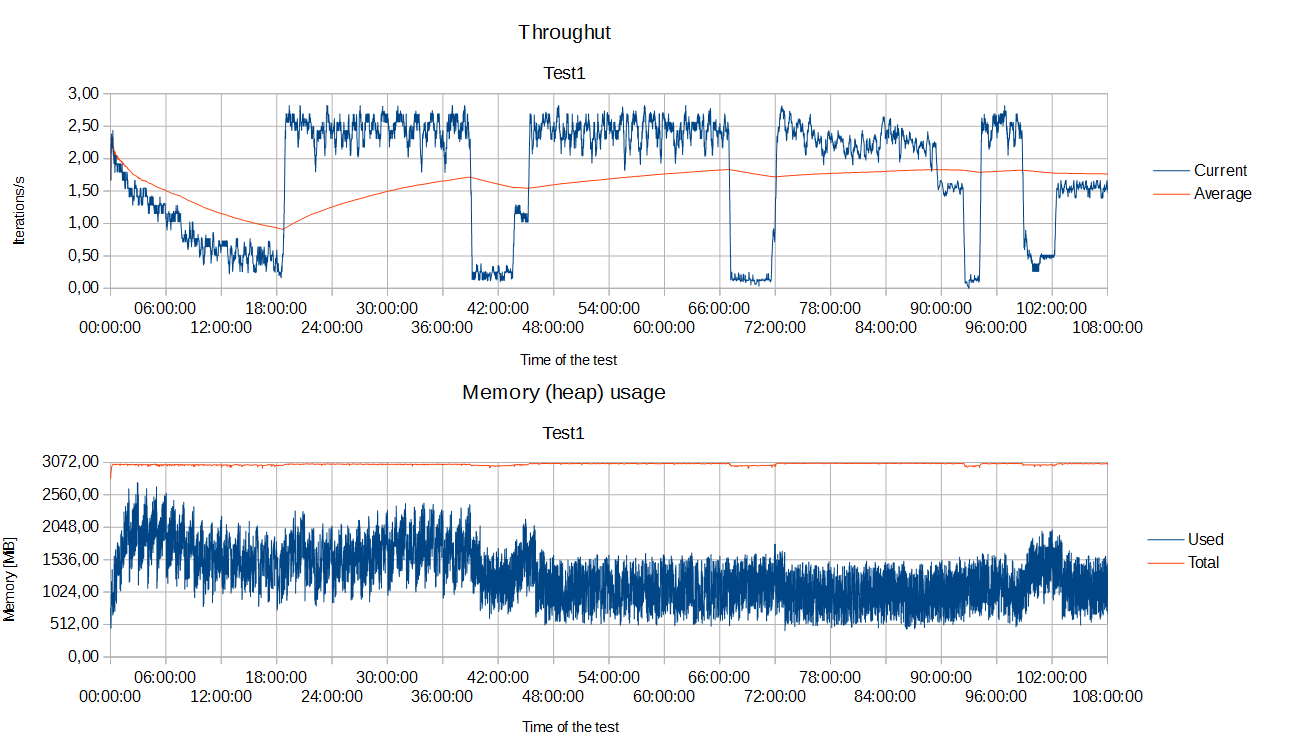
\includegraphics[scale=0.75, angle =90]{graphs.png}
\caption{Grafy}\label{grafy}
\end{figure}

\subsection{Dáta}

Pri optimalizácií dát pre potreby vykresľovania do grafov, bude používaný formát súboru CSV, ktorý môžeme previesť do podoby tabuľky.

Tabuľka  \ref{tab:Data} ukazuje dáta vygenerované nástrojom PerfCake za 20 minút, testovala sa priepustnosť softvéru v iteráciách za sekundu a využitie pamäte v megabajtoch. Pri vytváraní algoritmu budeme pracovať len s dátami, ktoré boli vytvorené pri testovaní týchto dvoch vlastností softvéru. Pri priepustnosti sa počíta priemer za časovú jednotku (current) a tiež priemer za niekoľko časových jednotiek (average), časová jednotka a veľkosť okna, s ktorými sa bude počíta sa 
dá nastaviť v scenári, pri dátach s tabuľky je to minúta a 15 záznamov. Priemer sa začína počítať, keď sa naplní okno a potom už pre každý ďalší záznam. 

Pri testovaní využívania pamäte sa zaznamenáva použitá (used) a celková pamäť (total). Celková pamäť, je pamäť, ktorú si  JVM alokuje a použitá pamäť je pamäť, ktorú naozaj využije - celková mínus voľná pamäť. Viac o pamäti v JVM sa čitateľ dozvie v oficiálnej dokumentácií(http://docs.oracle.com/javase/8/docs/api/java/lang/Runtime.html).

V popisovanej tabuľke sú dáta zaznamenané za 20 min, v praxi ale tie testy bežia väčšinou niekoľko desiatok hodín a teda tabuľky môžu dosahovať tisíce záznamov. Ukladať a následne spracovať takéto množstvo dát je pamäťovo aj časovo náročné a preto budem hľadať algoritmus, ktorý zmenší objem dát a zároveň neznehodnotí informáciu z nich vyplývajúcu, pri vykreslení do grafov.


\subsection{Grafy}

Pomocou grafu vieme často do mozgu preniesť oveľa viac informácií. 
Na obrázku  \ref{grafy} sú znázornené grafy z testov, ktoré bežali 108 hodín, a ktorých prvých 20 záznamov sme si ukázali v tabuľke  \ref{tab:Data}. Pre analýzu výsledku nie sú potrebné tak presné grafy, väčšinou je dôležitá hodnota okolo ktorej dáta v určitej časti grafu konvergujú, alebo či hodnoty veľmi ``skáču''. V bakalárskej práci budú tieto grafy upravené a následne porovnávané s grafmi, ktoré budú vykreslené z dát, na ktoré sa použije optimalizačný algoritmus.




%%%%%%%%%%%%%%%%%%%%%%%%%%%%%%%%%%%%
